\chapter{System Evaluation}
\section{Overview}
In this chapter we will look at actual performance and robustness of the system. We will also review how it compares to our initial goals and scope outlined in the Introduction chapter. We will also look at any technical limitations that we encountered during the project's life-cycle.

\section{Testing}
Throughout the project we incorporated multiple testing methodologies such as Functional and Non-functional testing. We will now look at the testing efforts and the results of said tests. More information and descriptions of what these methodologies involve can been found in the Methodology chapter.

\subsection{Functional Testing}
Functional testing focuses on the functional aspects of a system such as unit, integration and system testing.

\subsubsection{Unit Testing}
Unit testing was one of the first forms of testing we completed and was undertaken at a class level. It ensured the code, methods and classes written worked correctly individually. This was completed for both Unity and our Flask server.

\paragraph{Server Unit Testing}
To test the flask server which handles the AIML chatbot requests and sending data to the MongoDB server we used pytest. pytest is automatically imported in Python 3.6, and to run tests you simply put "test\_" before the method name and run the test file using "tests.py" in the command line. This allowed us to rapidly tests our code. To implement the testing some template test methods were setup which could be used multiple times by different tests. One was setup for the AIML requests and a second for the MongDB database uploads. Listing~\ref{lst:flasktest1} outlines the test method for AIML requests. This method takes in two parameters "test\_data" and "bot\_response". test\_data is the request to be sent to the server shown in listing~\ref{lst:flasktest2}. bot\_response is the response the AIML bot should return depending on the request sent. The template method shown in listing~\ref{lst:flasktest1}, uses these parameters, makes a call to the server and gets the response. The HTTP response code and AIML response is then checked using an assertion. If both assertions are true then the test passes. Response code 200 is a successful HTTP request. This testing allowed us to create a whole suite of tests for each type of persona and allowed us to test multiple responses at once. This improved our testing drastically as we didn't need to deploy the full application if we made changes to the server or AIML files.

\begin{lstlisting}[caption={pytest template method for testing AIML chatbot.},label={lst:flasktest1},language=python]

def test_predictResponse(test_data, bot_response):        
    response = app.test_client().post(
        '/request',
        data=json.dumps(test_data),
        content_type='application/json',
    )

    data = response.get_data()

    assert response.status_code == 200
    assert data == bot_response

\end{lstlisting}

\begin{lstlisting}[caption={pytest AIML runner methods which call template methods.},label={lst:flasktest2},language=python]

# AIML test runners.
def test_aiml_polite():
    test_data = {'sessionId': 1234, 'persona': 2, 'userInput': 'HELLO'}
    tests.test_predictResponse(test_data, "Hello Pleased to meet you!")

def test_aiml_neutral():
    test_data = {'sessionId': 1234, 'persona': 1, 'userInput': 'DO YOU HAVE A TICKET'}
    tests.test_predictResponse(test_data, "Here it is=1")

\end{lstlisting}

Postman was also used to to check the packets and debug errors. Postman is a piece of software focused on developing API's rapidly, and allows the user to send API requests to a server and check the response. We used this to unit test the server specifically without integrating it with the whole system. This contains the server URL hosted on PythonAnywhere with the method parameter "/request" defined in the flask server implementation. Attached with the request is form data which includes the session id, persona, speech input and whether the passenger has a ticket. An example of this can be seen in figure~\ref{image:postman}. 

\begin{figure}[ht]
	\caption{Postman request example.}
	\label{image:postman}
	\centering
	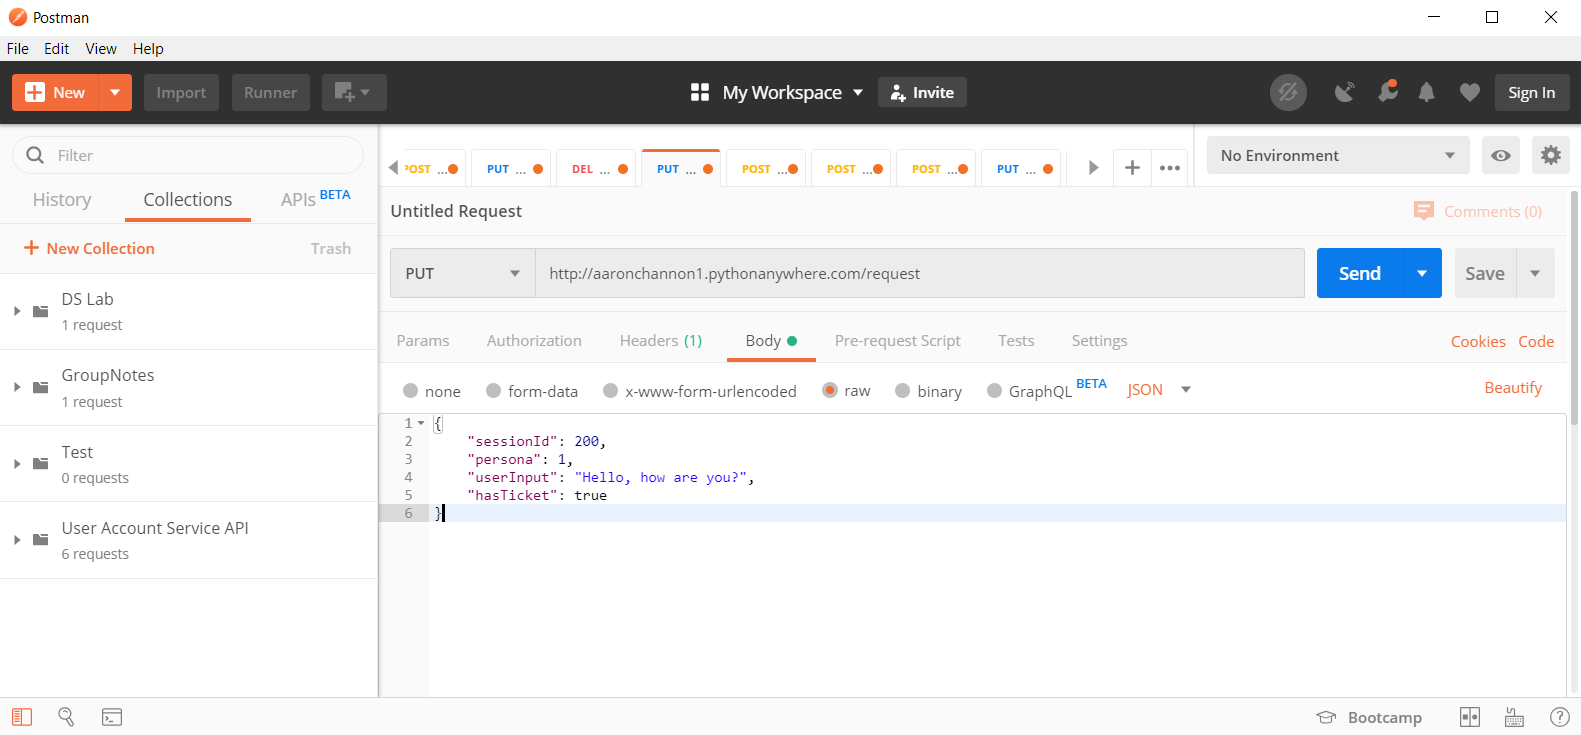
\includegraphics[width=1\textwidth]{Images/postman.PNG}
\end{figure}

\newpage

\subsubsection{Integration Testing}
Integration testing involves testing the system to insure it still works when adding new features, so it doesn't break other areas of the system. We implemented integration by testing for all aspects of the system to see if they still worked correctly on all iterative builds. As we have a lot of technologies working together seamlessly, integration tests were essential. After each new feature was added we would also run our unit tests again which are defined in listing~\ref{lst:flasktest1} and \ref{lst:flasktest2}. If they didn't pass then something was affecting the rest of the system. Due to the nature of our project user tests were also completed as integration tests, as bugs could develop from new features or when a new technology is added. One example of such an error was when adding Oculus Quest support and integrating it with the whole system. The Azure Speech Services would stop working once the application was closed and opened again. This was a major problem as the application could only be used once. From research of possible solutions and checking the error logs output by the Oculus Quest using LogCat, we came to a solution which we had thought would fix it. The Quest was throwing an error in regard to a .dll file it couldn't find. A number of people had a similar issue on a forum post, and the suggestion was to change the Unity version. To test this we built a new basic version of the project in Unity 2018, however the error still persisted when everything was added in. Going through each addition it was found that the error was caused by an Avatar game object that was added to the VR camera. This Avatar game object allows the user to see their own personal avatar in game connected to an Oculus account. It is useful for multiplayer games but not required for our application, but it is a standard addition to the supplied VR camera that Oculus provides so we would have never found this error without going through all possible options and integrating the Oculus support with the speech services.

\subsubsection{System Testing}
System testing is a black box testing methodology completed after integration testing to ensure the system meets the requirements. We implemented system testing by ensuring the application met the initial requirements outlined by the client in the Introduction Chapter. After each user, unit and integration test we would compare to our initial goals and see if we were meeting them. If it was a success we would move onto the next feature, but if not we would continue to develop the feature until it was meeting the required standard.

\subsection{Non-functional Testing}
Non-functional testing focuses the non-functional aspects of a system such as performance, usability and compatibility.

\subsubsection{Network/System Performance Testing}
Frame rate and response time where important for this project. We understood that the Oculus Quest would not perform as well as a gaming desktop but VR was a component that we could not remove from the project. To test the average frame rate we ran the project on both the Oculus and on a Gaming desktop. The average results can be seen in Figure~\ref{image:graph1}. The Oculus ran at around 55fps on average and the desktop ran at 110fps on average. We found that this was an appropriate amount of frames per second to ensure the user has a smooth experience. Regarding the response time, this can be seen in Figure~\ref{image:graph}. To obtain these results we interacted with an NPC once to see how fast it took them to respond. Both of us did this to get accurate results as our network speed are drastically different. Even though it took roughly 1.5 seconds to respond on a really bad internet connection we found that it did not take too much from the users experience.

\begin{figure}[h!]
	\caption{Response Time Graph.}
	\label{image:graph}
	\centering
	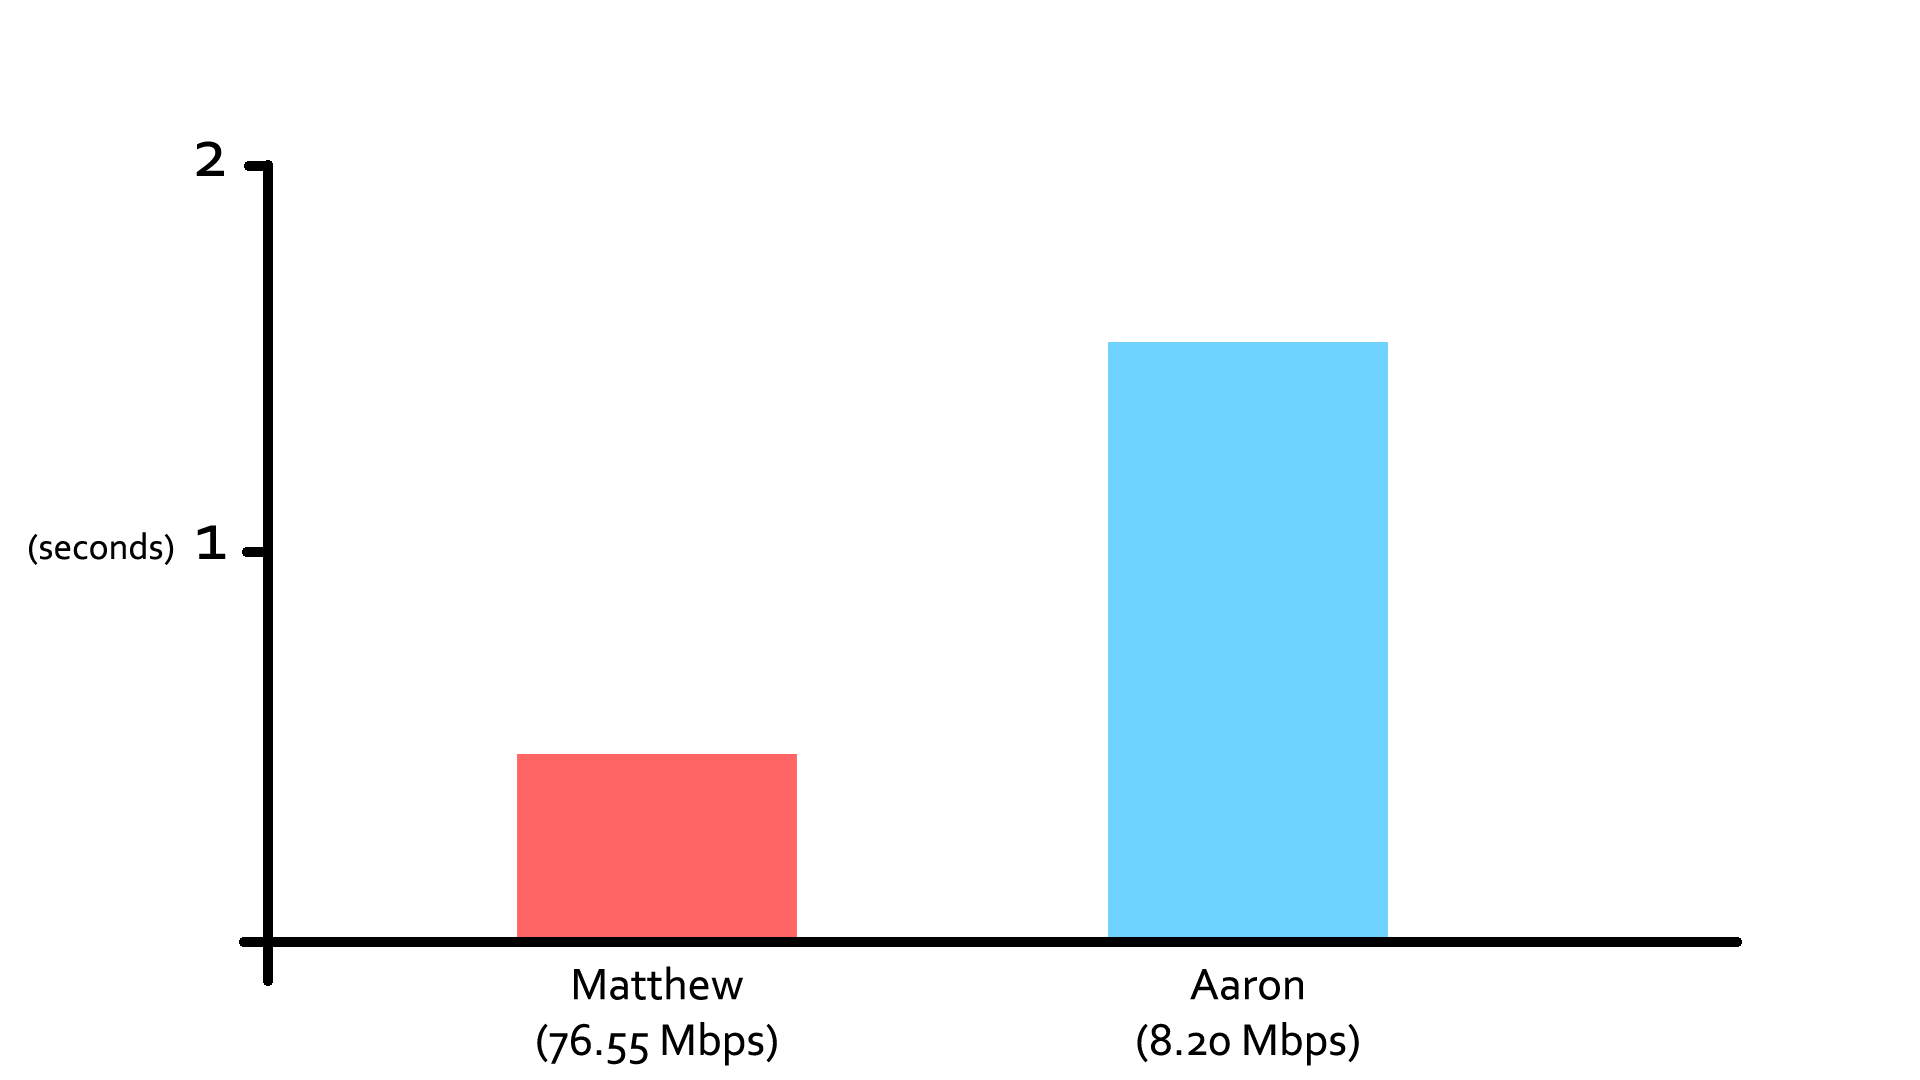
\includegraphics[width=1\textwidth]{Images/barchart connection.png}
\end{figure}

\begin{figure}[h!]
	\caption{Frame Rate Graph.}
	\label{image:graph1}
	\centering
	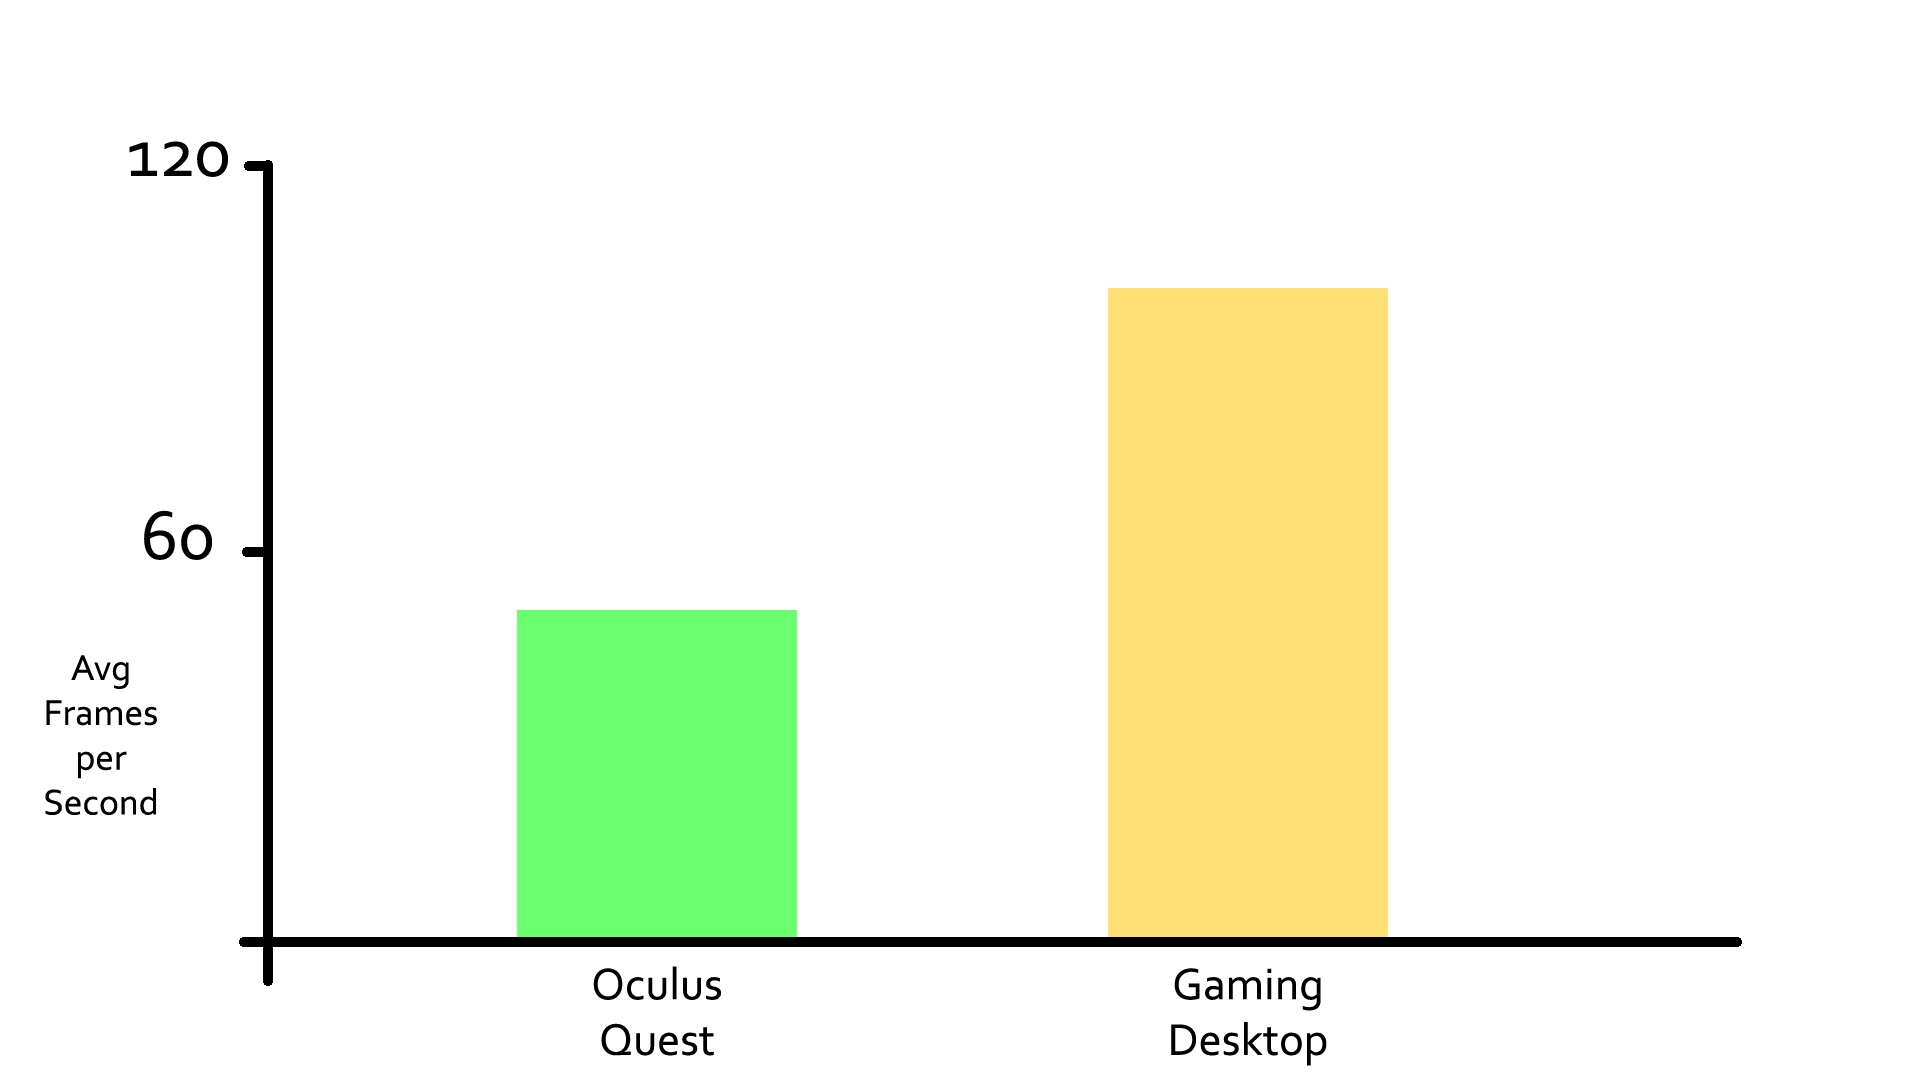
\includegraphics[width=1\textwidth]{Images/framerate.png}
\end{figure}
\clearpage

\subsubsection{Security Testing}
Security testing involves testing how secure the system is against unauthorized attacks. We implemented security measures regarding the server, deployment and database access. For example on the server, the database credentials were kept securely in an environments file and read in. This environment file is not published to our GitHub repository so there would be no unauthorized attempts to access the data saved. The same attitude was taken with the server and deployment for the AIML requests as the methods are purely GET/PUT requests which just return information and don't modify data.

\subsubsection{Usability Testing}
Usability testing involves measuring the ease of use from and end user’s perspective. This was vital to our game as it's a training experience, so we spent a lot of time working on improving usability of all controls, menus and game play. Throughout the development life cycle we tested the application with a number of friends and family along with our supervisor. From these tests we would collect their thoughts, ideas and improvements which helped us shape our final build. This testing was very important to us and really helped with the user experience design, the easy flow of conversation and simple interaction design between the user and the passengers. Examples of this include using speech to talk to the passengers, using a simple red, blue and green structured ring to display information about the passenger and displaying menu information on the players watch in virtual reality.

\subsubsection{Compatibility Testing}
Compatibility testing is a measure of how well a system works in different environments (Browsers, devices etc.). This was essential as we were developing the application to work on Android, Windows, and Oculus Quest VR. We initially developed for Windows for testing purposes but quickly started to develop for Android and the Oculus Quest as they both use the same Android build. Based on this it was essential that what we developed would be compatible with all platforms.

\section{Technological Limitations}

\subsection{Text To Speech Voices}
In an ideal world we would have real human voices replying to user but obviously this is impossible therefore being one of our technical limitations. However we found that Azure's AI voices were good enough to use when converting the AIML bot's text back to speech. We found a couple good voices that are included in Azure's API and decided to use those. There was a few other voices on the API that we tested and felt like they were not to the standard that we were looking for. Even though we were happy with the final product ideally we would have loved to have more dynamic and realistic voices that we could have added, but the current state of Azure's Speech API does not support this currently.

\subsection{Network Limitation}
As seen in Figure~\ref{image:graph} a high network speed is desired for the best user experience. The quicker the response time the more fluid the conversation appears to be. In an ideal world everyone would have high speed internet sadly this is not the case. If the user has slow internet e.g 10Mbps you could be waiting a second or two for a response which is not ideal. In our opinion this is a technical limitation that we can not control because we have optimised the transferring of data as best to our abilities so if a conversation with one of the NPCs is slow, it is all down to the user's internet connection. 

\subsection{Models \& Animations}
Ideally we would have ultra realistic models with 4K textures for all the NPCs and scene objects but we are not trained in modeling, texturing and animation so we made use of what we could find on the internet and the Unity asset store. If we did manage to have highly detailed models and texture we would find ourselves with another problem, that being performance on the Oculus Quest. If we had a VR headset that was not mobile we could have added better models, if we had them. Even though this is a technical limitation we were still extremely happy with the final state and aesthetic of the project.

\section{Completed Objectives}
Based on our goals/objectives from the introduction we believe we completed them all. Below is a list of our completed objectives.

\begin{itemize}
    \item We developed a project based on requirements that the client was happy with.
    \item We researched all the latest technologies so that the application would not be out-dated.
    \item We implemented a robust system based on our research.
    \item We created a project that we were happy with as well as the client.
\end{itemize}




